\chapter{Numerical Partial Differential Equations}
Partial differential equations (PDEs) are differential equations involving the partial
derivatives of an unknown multivariable function.  In many cases we are interested in
ultimately solving PDEs in terms of our usual three spatial dimensions along with an extra
dimension for time.  Since PDEs require a strong background in the notions of vector
calculus we'll start there.

\section{Quick Review -- Main Ideas from Vector Calculus}
Let's start with some basic review of multivariable calculus.
\begin{problem}
    With your partner answer each of the following questions. The main ideas in this
    problem {\it should} be review from multivariable calculus.  If you and your partner
    are stuck then ask another group. 
    \begin{enumerate}
        \item[(a)] What is a partial derivative (explain geometrically)
        \item[(b)] What is the gradient of a function? What does it tell us physically or geometrically? If
            $u(x,y)=x^2+\sin(xy)$ then what is $\nabla u$?
        \item[(c)] What is the divergence of a vector-valued function? What does it tell
            us physically or geometrically? If $F(x,y)=\left< \sin(xy), x^2+y^2\right>$
            then what is $\nabla \cdot F$?
        \item[(d)] If $u$ is a function of $x$, $y$, and $z$ then what is $\nabla \cdot
            \nabla u$?
        \item[(e)] What is the divergence theorem? (ok \ldots go ahead and use the
            internet for this one) Be able to explain what you find. 
    \end{enumerate}
\end{problem}

Now that you've realized that you don't recall most of your multivariable calculus, let's
simply recap.
\begin{definition}[Definitions from Multivariable Calculus]
    The following are a few of the primary definitions and theorems from multivariable
    calculus.
    \begin{itemize}
        \item The {\bf del} or {\bf grad} operator, $\nabla$, is a vector operator 
            \[ \nabla = \left< \frac{\partial}{\partial x} \, , \,
                \frac{\partial}{\partial y} \, , \, \frac{\partial}{\partial z} \right>.
            \]
        \item The {\bf gradient} of a multivariable function $u(x,y,z)$ is the vector
            \[ \nabla u = \left< \frac{\partial u}{\partial x} \, , \,
                \frac{\partial u}{\partial y} \, , \, \frac{\partial u}{\partial z}
            \right>. \]
        \item The {\bf divergence} of a vector valued function $F = \left< F_1, F_2,
            F_3\right>$ is the scalar
            \[ \nabla \cdot F = \pd{F_1}{x} + \pd{F_2}{y} + \pd{F_3}{z}. \]
        \item The {\bf curl} of a vector valued function $F = \left< F_1, F_2,
            F_3\right>$ is the vector
            \[ \nabla \times F = \begin{vmatrix} \hat{i} & \hat{j} & \hat{k} \\ \pd{ }{x}
                & \pd{ }{y} & \pd{ }{z} \\ F_1 & F_2 & F_3 \end{vmatrix} = \left<
        \pd{F_3}{y} - \pd{F_2}{z} \, , \, -\left( \pd{F_3}{x} - \pd{F_1}{z} \right) \, ,
    \, \pd{F_2}{x} - \pd{F_1}{y} \right>.\] 
        \item The {\bf Laplacian} of a multivariable function $u(x,y,z)$ is the scalar
            \[ \nabla \cdot \nabla u = \pdd{u}{x} + \pdd{u}{y} + \pdd{u}{z}. \]
        \item The {\bf divergence theorem} states that the flux of a vector field out of closed body is the
            same as the integral of the divergence of the vector field within the body.
            \[ \iint F \cdot n dA = \iiint \nabla \cdot F dV. \]
    \end{itemize}
\end{definition}

\newpage\section{An Intuitive Introduction to some Common PDEs}
To build intuition for partial differential equations we'll first start with your
intuition with ordinary differential equations.  Let's consider the really simple ODE $y'
= y$.  We can verbalize this problems with the phrase {\it the rate of change of $y$ is
equal to the current value of $y$}, and we can use this phrase, along with our
understanding of linear approximation from Calculus, to build intuition about
how the value of $y$ propogates in time.  
If we start with a value of $y(0) = 0.5$ then after 1 unit of time passes we have a reasonable
guess for the value of $y$ based on our understanding of slope:
\[ y(1) \approx 0.5 + (1)(0.5) = 1. \]
Similarly we can propogate forward 1 unit of time again to get 
\[ y(2) \approx 1 + 1(1) = 2, \]
and we can continue this to get 
\begin{center}
    \begin{tabular}{|c||c|c|c|c|c|c|}
        \hline
        Time & 0 & 1 & 2 & 3 & 4 & $\cdots$ \\\hline
        $y$ & 0.5 & 1 & 2 & 4 & 8 & $\cdots$ \\ \hline
    \end{tabular}
\end{center}
We also know that this isn't quite correct since the solution to the differntial equation
is $y(t) = 0.5 e^t$.  In Figure \ref{fig:intuition_odes} we can see, however, that our intuitive guesses get
us somewhat close to the basic behavior of the differential equation but clearly miss the
finer details associated with the exact curvature. 
\begin{figure}[ht!]
    \begin{center}
        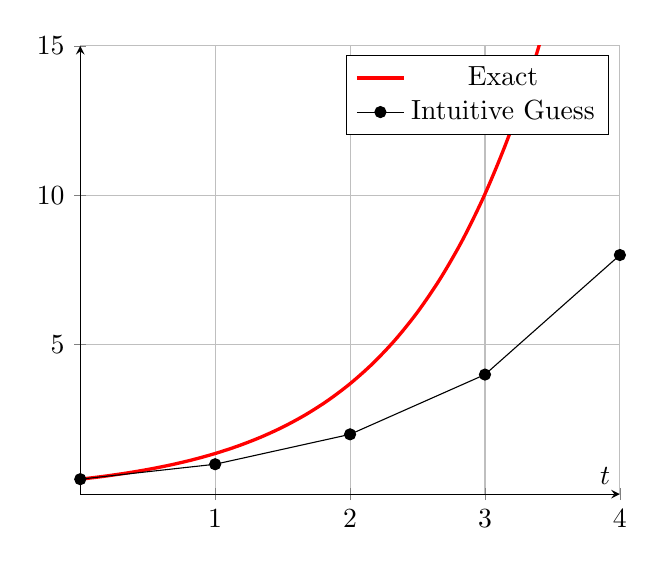
\begin{tikzpicture}
            \begin{axis}[axis lines=center, grid, domain=0:4, xlabel={$t$}, ymax=15,
                ymin=0]
                \addplot[smooth, very thick, red] {0.5*exp(x)};
                \addlegendentry{Exact};
                \addplot[mark=*, color=black] coordinates{(0,0.5)(1,1)(2,2)(3,4)(4,8)};
                \addlegendentry{Intuitive Guess};
            \end{axis}
        \end{tikzpicture}
    \end{center}
    \caption{The analytic solution to $y'=y$ and the points given by calculus intuition.}
    \label{fig:intuition_odes}
\end{figure}

We're going to use this same idea to build intuition for some of the most basic partial
differential equations.  In these partial differential equations we have two variables:
$t=$ time and $x=$ a single spatial dimension.  

\begin{problem}\label{prob:heat_intuition_1}
    Let $u(t,x)$ be the concentration of a quantity at time $t$ and spatial location $x$.
    The quantity might be something like heat or chemical concentration.
    We will let $x \in [0,1]$ and we assume that at time $t=0$ we have $u(0,x) = \sin(2\pi
    x)$ as shown in the plot below.  Use the phrase 
    \begin{quote}
        {\it the time rate of change of concentration is equal to the concavity of the
        concentration function}
    \end{quote}
    to give several plots showing how the concentration evolves in time. The initial
    condition function $u(0,x)$ is shown in each plot for reference.  Think of this as
    creating four frames in an animation.
    \begin{center}
        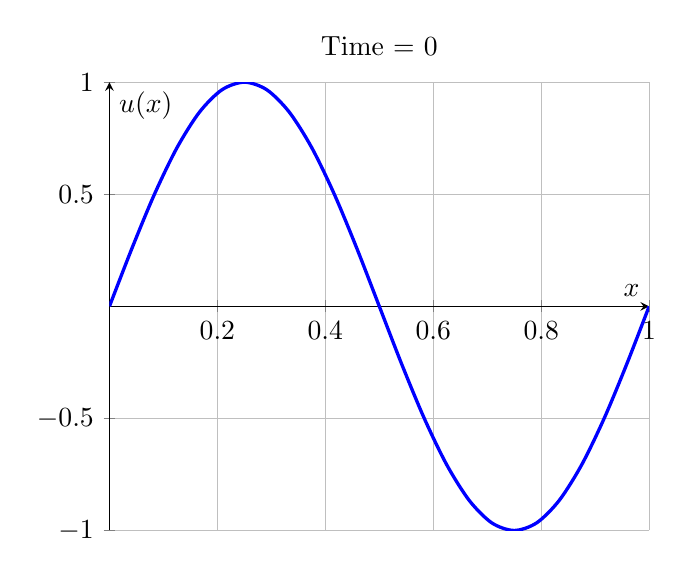
\begin{tikzpicture}
            \begin{axis}[axis lines=center, grid, domain=0:1, xlabel={$x$},
                ylabel={$u(x)$}, title={Time = 0}]
                \addplot[smooth, very thick, blue] {sin(2*pi*deg(x))};
            \end{axis}
        \end{tikzpicture}\\
        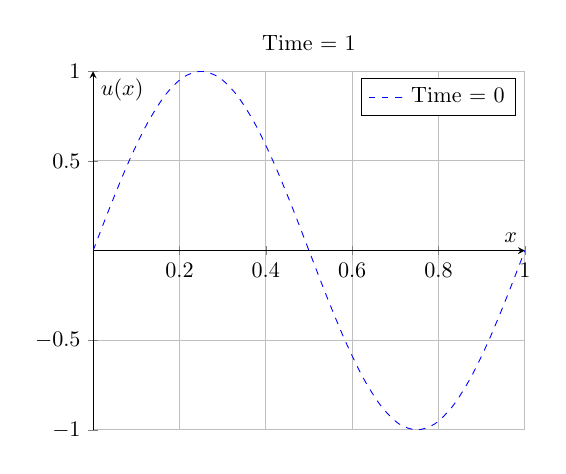
\begin{tikzpicture}[scale=0.8]
            \begin{axis}[axis lines=center, grid, domain=0:1, xlabel={$x$},
                ylabel={$u(x)$}, title={Time = 1}]
                \addplot[smooth, blue, dashed] {sin(2*pi*deg(x))};
                \addlegendentry{Time = 0};
            \end{axis}
        \end{tikzpicture}
        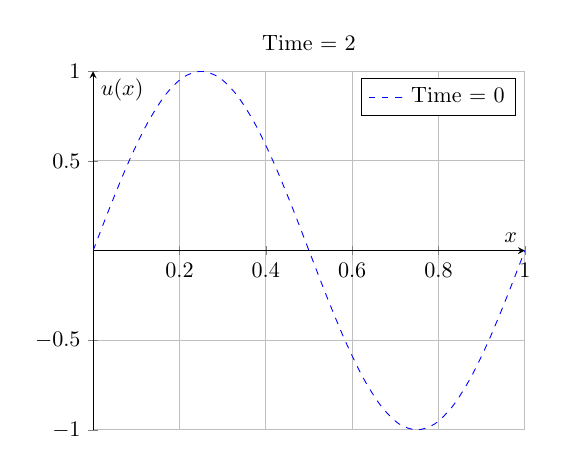
\begin{tikzpicture}[scale=0.8]
            \begin{axis}[axis lines=center, grid, domain=0:1, xlabel={$x$},
                ylabel={$u(x)$}, title={Time = 2}]
                \addplot[smooth, blue, dashed] {sin(2*pi*deg(x))};
                \addlegendentry{Time = 0};
            \end{axis}
        \end{tikzpicture}
        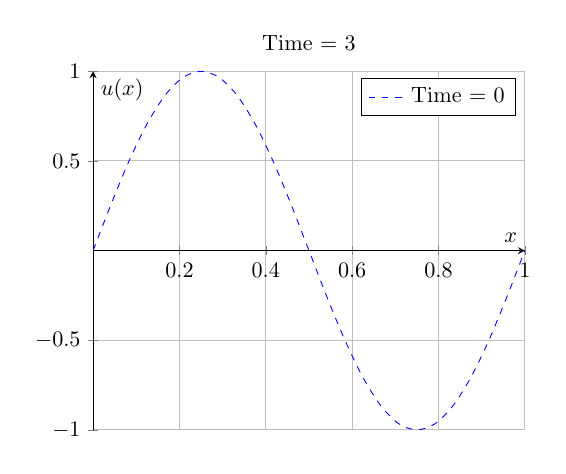
\begin{tikzpicture}[scale=0.8]
            \begin{axis}[axis lines=center, grid, domain=0:1, xlabel={$x$},
                ylabel={$u(x)$}, title={Time = 3}]
                \addplot[smooth, blue, dashed] {sin(2*pi*deg(x))};
                \addlegendentry{Time = 0};
            \end{axis}
        \end{tikzpicture}
        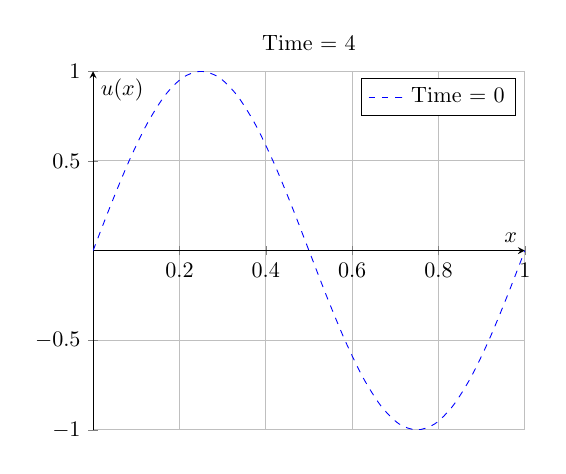
\begin{tikzpicture}[scale=0.8]
            \begin{axis}[axis lines=center, grid, domain=0:1, xlabel={$x$},
                ylabel={$u(x)$}, title={Time = 4}]
                \addplot[smooth, blue, dashed] {sin(2*pi*deg(x))};
                \addlegendentry{Time = 0};
            \end{axis}
        \end{tikzpicture}
    \end{center}
\end{problem}


\begin{problem}\label{prob:heat_intuition_2}
    Which of the following differential equations corresponds to the phrase 
        {\it ``the time rate of change of concentration is equal to the concavity of the
        concentration function''}?
        \[ \pd{u}{t} = -\pd{u}{x}, \qquad \pd{u}{t} = \pdd{u}{x}, \quad \text{or} \quad \pdd{u}{t} =
        \pdd{u}{x} \]
        Explain your reasoning clearly.
\end{problem}

\begin{problem}
    Based on your answer to Problem \ref{prob:heat_intuition_1} you should now have an intuitive
    sense for the behavior of the solution to the partial differential equation that you
    identified in Problem \ref{prob:heat_intuition_2}.  This equation is called the {\bf Heat
    Equation} or the {\bf Diffusion Equation}.  Give context to the physical process that is being
    described by this equation.
\end{problem}

\begin{problem}
    How would your answer to Problem \ref{prob:heat_intuition_1} change if we were to
    modify the heat equation to 
    \[ \pd{u}{t} = 0.5 \pdd{u}{x}? \]
    What about 
    \[ \pd{u}{t} = 2 \pdd{u}{x}? \]
\end{problem}

\begin{problem}
    The 1D Heat Equation is given as 
    \[ \pd{u}{t} = D \pdd{u}{x}. \]
    What does the parameter $D$ control in terms of the physics of the problem?
\end{problem}



\begin{problem}\label{prob:wave_intuition_1}
    Let $u(t,x)$ be the position of a string or cable at time $t$ and spatial location $x$.
    We will let $x \in [0,1]$ and we assume that at time $t=0$ we have $u(0,x) = \sin(2\pi
    x)$ as shown in the plot below.  Use the phrase 
    \begin{quote}
        {\it the acceleration of each point on the string is equal to the concavity
        of the string}
    \end{quote}
    to give several plots showing how the concentration evolves in time. The initial
    condition function $u(0,x)$ is shown in each plot for reference.  Think of this as
    creating four frames in an animation.
    \begin{center}
        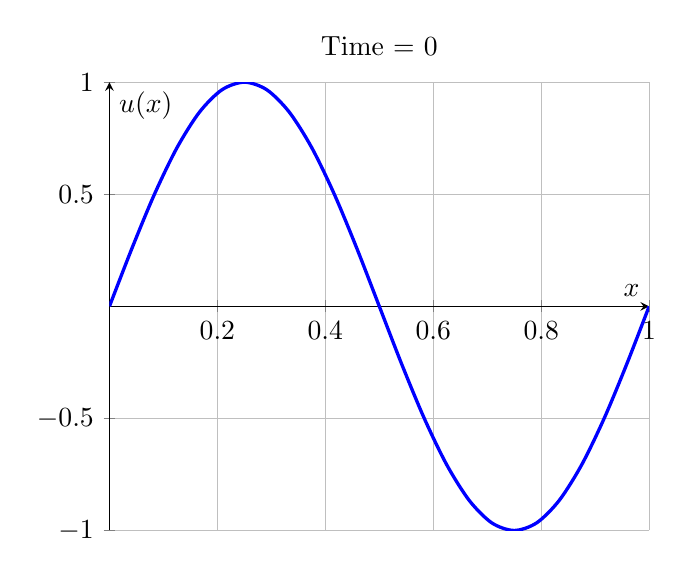
\begin{tikzpicture}
            \begin{axis}[axis lines=center, grid, domain=0:1, xlabel={$x$},
                ylabel={$u(x)$}, title={Time = 0}]
                \addplot[smooth, very thick, blue] {sin(2*pi*deg(x))};
            \end{axis}
        \end{tikzpicture}\\
        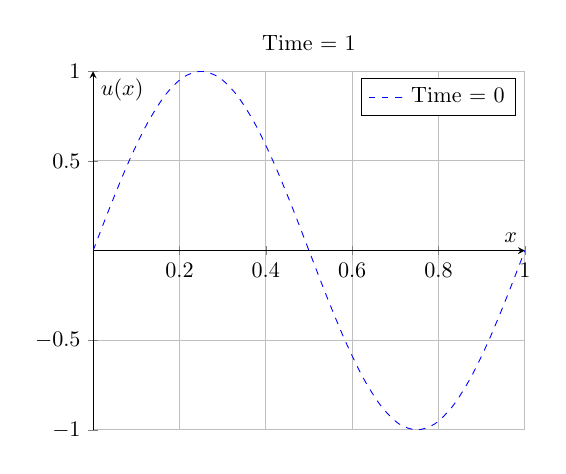
\begin{tikzpicture}[scale=0.8]
            \begin{axis}[axis lines=center, grid, domain=0:1, xlabel={$x$},
                ylabel={$u(x)$}, title={Time = 1}]
                \addplot[smooth, blue, dashed] {sin(2*pi*deg(x))};
                \addlegendentry{Time = 0};
            \end{axis}
        \end{tikzpicture}
        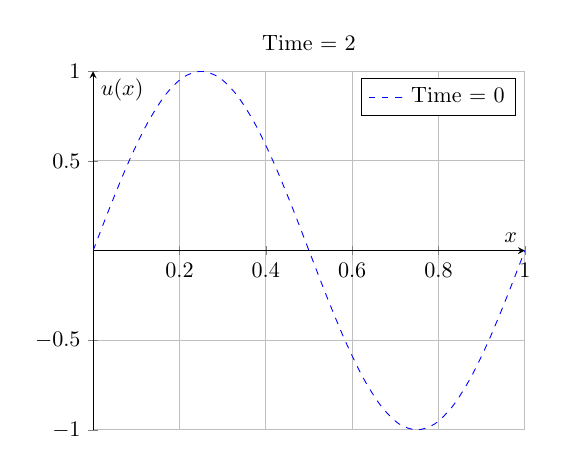
\begin{tikzpicture}[scale=0.8]
            \begin{axis}[axis lines=center, grid, domain=0:1, xlabel={$x$},
                ylabel={$u(x)$}, title={Time = 2}]
                \addplot[smooth, blue, dashed] {sin(2*pi*deg(x))};
                \addlegendentry{Time = 0};
            \end{axis}
        \end{tikzpicture}
        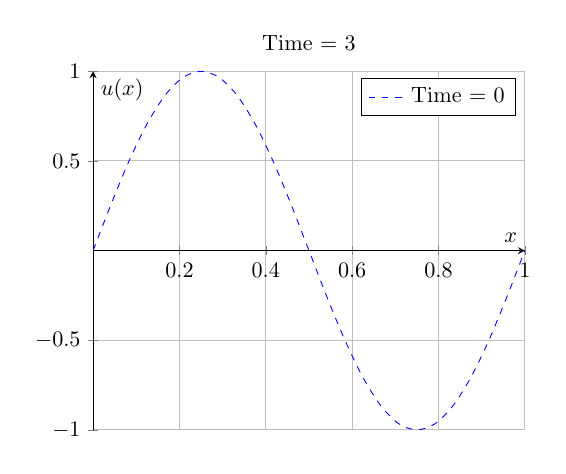
\begin{tikzpicture}[scale=0.8]
            \begin{axis}[axis lines=center, grid, domain=0:1, xlabel={$x$},
                ylabel={$u(x)$}, title={Time = 3}]
                \addplot[smooth, blue, dashed] {sin(2*pi*deg(x))};
                \addlegendentry{Time = 0};
            \end{axis}
        \end{tikzpicture}
        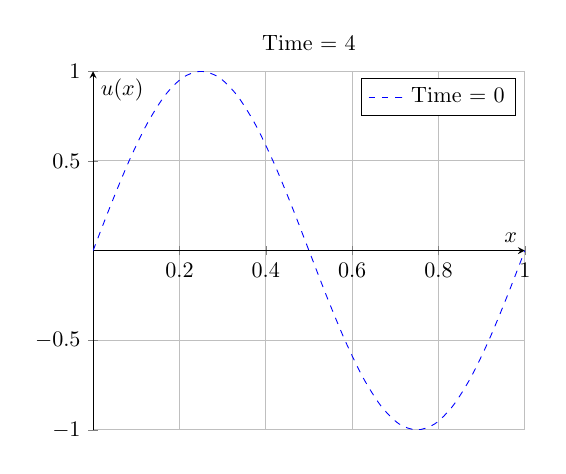
\begin{tikzpicture}[scale=0.8]
            \begin{axis}[axis lines=center, grid, domain=0:1, xlabel={$x$},
                ylabel={$u(x)$}, title={Time = 4}]
                \addplot[smooth, blue, dashed] {sin(2*pi*deg(x))};
                \addlegendentry{Time = 0};
            \end{axis}
        \end{tikzpicture}
    \end{center}
\end{problem}


\begin{problem}\label{prob:wave_intuition_2}
    Which of the following differential equations corresponds to the phrase 
        {\it ``the acceleration of each point on the string is equal to the concavity
        of the string''}?
        \[ \pd{u}{t} = -\pd{u}{x}, \qquad \pd{u}{t} = \pdd{u}{x}, \quad \text{or} \quad \pdd{u}{t} =
        \pdd{u}{x} \]
        Explain your reasoning clearly.
\end{problem}

\begin{problem}
    Based on your answer to Problem \ref{prob:wave_intuition_1} you should now have an
    intuitive sense for the behavior of the solution to the partial differential equation
    that you identified in Problem \ref{prob:wave_intuition_2}.  This equation is called
    the {\bf Wave Equation}.  Give context to the physical process that is being described
    by this equation.
\end{problem}


\begin{problem}
    How would your answer to Problem \ref{prob:wave_intuition_1} change if we were to
    modify the wave equation to 
    \[ \pdd{u}{t} = 0.5 \pdd{u}{x}? \]
    What about 
    \[ \pdd{u}{t} = 2 \pdd{u}{x}? \]
\end{problem}

\begin{problem}
    The 1D Wave Equation is given as 
    \[ \pdd{u}{t} = \alpha^2 \pdd{u}{x}. \]
    What does the parameter $\alpha^2$ control in terms of the physics of the problem?
\end{problem}



\newpage\section{An Analytic Introduction to Conservation Law PDEs}
In the previous section
we just gave you the PDEs without any proof of where they came from.  In this section
we'll give a more analytic introduction to most of the primary partial
differential equations of interest in basic mathematical physics.  We will make reference
to Fick's Law for mass transport and Fourier's Law for thermal transport, so interested
readers should dig deeper by examining the relevant Wikipedia pages.
  
Conservation laws pervade all of physics -- conservation of energy, conservation of
momentum, and conservation of mass.  These laws are sometimes stated colloquially as
{\it energy (or momentum or mass) can neither be created nor destroyed}, but this phrase
is not super helpful mathematically.  We start this section with a brief mathematical
derivation of a {\it general conservation law} to further clarify what we mean
mathematically.  The resulting general conservation law will be a
partial differential equation that can be used to mathematically express the physical laws
of conservation of mass, momentum, or
energy.

Let $u$ be the quantity you are trying to conserve, $\bq$ be the flux of that quantity,
and $f$ be any source of that quantity.  For example, if we are to derive a conservation
of energy equation, $u$ might be energy, $\bq$ might be temperature flux, and $f$ might be
a temperature source (or sink).

\subsection*{Derivation of General Balance Law}
Let $\Omega$ be a fixed volume and denote the boundary of this volume by $\partial
\Omega$. The rate at which $u$ is changing in time throughout $\Omega$ needs to be
balanced by the rate at which $u$ leaves the volume plus any sources of $u$.
Mathematically, this means that
\begin{flalign}
    \pd{ }{t} \iiint_{\Omega} u dV = -\iint_{\partial \Omega} \bq \cdot n dA +
    \iiint_\Omega f dV.
    \label{eqn:global_balance}
\end{flalign}
This is a global balance law in the sense that it holds for all volumes $\Omega$.  The
mathematical 
troubles here are two fold: (1) there are many integrals, and (2) there are really two variables
($u$ and $q$ since $f=f(u,x,t)$) so the equation is not closed.  In order to mitigate
that fact we apply the divergence theorem to the first term on the right-hand side of
\eqref{eqn:global_balance} to get
\begin{flalign}
    \pd{ }{t} \iiint_{\Omega} u dV = -\iiint_{\Omega} \nabla \cdot \bq dV +
    \iiint_\Omega f dV.
    \label{eqn:global_balance2}
\end{flalign}

Gathering all of the terms on the right of \eqref{eqn:global_balance2}, interchanging the integral and the derivative on
the left (since the volume is not changing in time), and rewriting gives
\begin{flalign}
    \iiint_\Omega \left( \pd{u}{t} + \nabla \cdot \bq \right) dV = \iiint_\Omega f dV
    \label{eqn:global_balance3}
\end{flalign}
If we presume that this equation holds for all volumes $\Omega$ then the integrands must
be equal and we get the local balance law
\begin{flalign}
    \pd{u}{t} + \nabla \cdot \bq = f.
    \label{eqn:local_balance}
\end{flalign}

Equation \eqref{eqn:local_balance} is an expression of the balances of changes in time to
changes in space of a conserved quantity such as mass, momentum, or energy.  What remains
is to make clear the meaning and functional form of the flux $\bq$ and the source function
$f$.

\subsection*{Simplification of the Local Balance Law}
In equation \eqref{eqn:local_balance} it is often assumed that the system is free of
external sources.  In this case we set $f$ to zero and obtain the source-free balance law
\begin{flalign}
    \pd{u}{t} + \nabla \cdot \bq = 0.
    \label{eqn:local_source_free}
\end{flalign}
It is this form of balance law where many of the most interesting and important partial
differential equations come from.  In particular consider the following two cases: mass
balance and energy balance.
\subsection*{Mass Balance}
In mass balance we take $u$ to either be the density of a substance (e.g. in the case of
liquids) or the concentration of a substance in a mixture (e.g. in the case of
gasses). If $C$ is the mass concentration of a substance in a gas then the flux of that
substance is given via Fick's Law as
\begin{flalign}
    \bq = -k \nabla C.
    \label{eqn:fick}
\end{flalign}
Combining \eqref{eqn:fick} with \eqref{eqn:local_source_free} (and assuming that $k$ is
independent of space, time, and concentration) gives
\begin{flalign}
    \pd{C}{t} = k \nabla \cdot \nabla C. 
    \label{eqn:fick2_simp}
\end{flalign}
In the presence of external sources of mass, \eqref{eqn:fick2_simp} is
\begin{flalign}
    \pd{C}{t} = k \nabla \cdot \nabla C + f(x).
    \label{eqn:fick3}
\end{flalign}
Expanding the Laplacian operator on the right-hand side of \eqref{eqn:fick3} we get
\begin{flalign}
    \pd{C}{t} = k\left( \pdd{C}{x} + \pdd{C}{y} + \pdd{C}{z} \right) + f(x)
    \label{eqn:fick3_expanded}
\end{flalign}
where the reader should note that this can be easily simplified in 1 or 2 spatial
dimensions.
% \begin{problem}
%     What does \eqref{eqn:fick3} equation look like in terms of spatial derivatives on the
%     right-hand side?
%     \begin{flalign*}
%         \pd{C}{t} &= \underline{\hspace{2in}} \quad \text{(1 Spatial Dimension)} \\
%         \pd{C}{t} &= \underline{\hspace{2in}} \quad \text{(2 Spatial Dimensions)} \\
%         \pd{C}{t} &= \underline{\hspace{2in}} \quad \text{(3 Spatial Dimensions)}
%     \end{flalign*}
% \end{problem}

\subsection*{Energy Balance}
The energy balance equation is essentially the same as the mass balance equation.  If $u$
is temperature then the flux of temperature is given by Fourier's Law for heat conduction
\begin{flalign}
    \bq = -k\nabla T.
    \label{eqn:fourier}
\end{flalign}
Making the same simplifications as in the mass balance equation we arrive at
\begin{flalign}
    \pd{T}{t} = k \nabla \cdot \nabla T.
    \label{eqn:fourier2}
\end{flalign}
In the presence of external sources of heat, \eqref{eqn:fourier2} becomes
\begin{flalign}
    \pd{T}{t} = k \nabla \cdot \nabla T + f(x).
    \label{eqn:fourier3}
\end{flalign}
Expanding the Laplacian operator on the right-hand side of \eqref{eqn:fourier3} we get
\begin{flalign}
    \pd{T}{t} = k\left( \pdd{T}{x} + \pdd{T}{y} + \pdd{T}{z} \right) + f(x)
    \label{eqn:fourier3_expanded}
\end{flalign}
where the reader should note that this can be easily simplified in 1 or 2 spatial
dimensions.
% \begin{problem}
%     What does \eqref{eqn:fourier3} equation look like in terms of spatial derivatives on the
%     right-hand side?
%     \begin{flalign*}
%         \pd{T}{t} &= \underline{\hspace{2in}} \quad \text{(1 Spatial Dimension)} \\
%         \pd{T}{t} &= \underline{\hspace{2in}} \quad \text{(2 Spatial Dimensions)}\\
%         \pd{T}{t} &= \underline{\hspace{2in}} \quad \text{(3 Spatial Dimensions)}
%     \end{flalign*}
% \end{problem}



\subsection*{Laplace's Equation and Poisson's Equation}
Equations \eqref{eqn:fick3} and \eqref{eqn:fourier3} are the same partial differential
equation for two very important physical phenomenon; mass and heat transfer.  In the case
where time is allowed to run to infinity and no external sources of mass or energy are
included these equations reach a steady state solution (no longer changing in time) and we
arrive at Laplace's Equation
\begin{flalign}
    \nabla \cdot \nabla u = 0.
    \label{eqn:laplace}
\end{flalign}
Laplace's equation is actually a statement of minimal energy as well as steady state heat
or temperature.  We can see this since entropy always drives systems from high energy to
low energy, and if we have reached a steady state then we must have also reached a surface
of minimal energy.

Equation \eqref{eqn:laplace} is sometimes denoted as $\nabla \cdot \nabla u = \nabla^2 u =
\Delta u$, and in terms of the partial derivatives it is written as
\begin{flalign*}
    \pdd{u}{x} + \pdd{u}{y} + \pdd{u}{z} = 0.
% V    0 &= \underline{\hspace{2in}} \quad \text{(1 Spatial Dimension)} \\
%     0 &= \underline{\hspace{2in}} \quad \text{(2 Spatial Dimensions)} \\
%     0 &= \underline{\hspace{2in}} \quad \text{(3 Spatial Dimensions)} 
\end{flalign*}

If there is a time-independent external source the right-hand side of
\eqref{eqn:laplace} will be non-zero and we arrive at Poisson's equation:
\begin{flalign}
    \nabla \cdot \nabla u = -f(x).
    \label{eqn:poisson}
\end{flalign}
Note that the negative on the right-hand side comes from the fact that
$\pd{u}{t} = k \nabla \cdot \nabla u + f(x)$ and $\pd{u}{t} \to 0$.  Technically we are
absorbing the constant $k$ into $f$ (that is ``$f$'' is really ``$f/k$'').  Also
note that in many instances the value of $k$ is not constant and cannot therefore be pulled
out of the derivative without a use of the product rule.

Let's summarize:
\begin{center}
    \begin{tabular}{|c|c|c|}
        \hline
        Name of PDE & PDE & What the PDE Models \\ \hline \hline
        The Heat Equation & $\ds \pd{u}{t} = k \nabla \cdot \nabla u + f(x)$ & Diffusion \\
        Laplace's Equation & $\ds k \nabla \cdot \nabla u =-f(x)$ & Minimal Energy
        Surfaces \\
%         The Wave Equation & $\ds \pdd{u}{t} = k \nabla \cdot \nabla u + f(x)$ & Wave
%         phenomena \\
        \hline
    \end{tabular}
\end{center}

Further discussion of the origins of the wave equation and other interesting PDE's is left
to the reader.


\newpage\section{Boundary Conditions}
When we were solving ODEs we typically needed initial conditions to tell us where the
solutions starts at time 0.  Since PDEs require both spatial and temporal information we
need to tell the differential equation how to behave both at time zero and on the
boundaries of the domain.  

\begin{definition}
    Let's say that we want to solve the 1D heat equation $u_t = k u_{xx}$ on the domain $x
    \in [0,1]$.  
    \begin{itemize}
        \item The initial condition is a function $\eta(x)$ where $u(0,x) = \eta(x)$.  In
            other words, we are dictating the value of $u$ at every point $x$ at time
            $t=0$. 
        \item The boundary conditions are restrictions for how the solution behaves at
            $x=0$ and $x=1$ (for this problem).  
            \begin{itemize}
                \item If the value of the solution $u$ at the boundary is either a fixed value or a fixed
                    function of time then we call the boundary condition a {\bf Dirichlet
                    boundary condition.}  For example, $u(t,0) = 1$ and $u(t,1) = 5$ are
                    Dirichlet boundary conditions for this problem.  They state that the
                    value of the temperature is fixed at these points.
                \item If the value of the solution $u$ depends on the rate of change of
                    $u$ at the boundary then we call the boundary condition a {\bf Neumann
                    boundary condition.}  For example, $\pd{u}{x}(t,0) = 0$ and
                    $\pd{u}{x}(t,1) = 0$ are Neumann boundary conditions for this problem.
                    They state that the flux of temperature is fixed at the boundaries.
            \end{itemize}
            
    \end{itemize}
\end{definition}

Let's play with a couple problems that should help to build your intuition about boundary
conditions in PDEs.  Again, we will do this graphically instead of numerically.
\begin{problem}
    Consider solving the heat equation $u_t = u_{xx}$ in 1 spatial dimension.  It will
    be helpful to reconsider Problem \ref{prob:heat_intuition_1} for this problem.
    \begin{enumerate}
        \item[(a)] In Problem \ref{prob:heat_intuition_1} we didn't explicitly state the
            boundary conditions.  What type of boundary conditions were they?  How can
            you tell?
        \item[(b)] What if we take the initial condition for the 1D heat equation to be
            $u(0,x) = \cos(2\pi x)$ and enforce the conditions $\pd{u}{x}\Big|_{x=0} = 0$
            and $u(t,1) = 1$.
            What types of boundary conditions are these?  Draw a collection of pictures
            showing the expected evolution of the heat equation with these boundary
            conditions.
    \end{enumerate}
\end{problem}






\begin{problem}
    Consider solving the wave equation $u_{tt} = u_{xx}$ in 1 spatial dimension.  It will
    be helpful to reconsider Problem \ref{prob:wave_intuition_1} for this problem.
    \begin{enumerate}
        \item[(a)] In Problem \ref{prob:wave_intuition_1} we didn't explicitly state the
            boundary conditions.  What type of boundary conditions were they?  How can
            you tell?
        \item[(b)] What if we take the initial condition for the 1D wave equation to be
            $u(0,x) = \cos(2\pi x)$ and enforce the conditions $\pd{u}{x}\Big|_{x=0} = 0$
            and $u(t,1) = 1$.
            What types of boundary conditions are these?  Draw a collection of pictures
            showing the expected evolution of the heat equation with these boundary
            conditions.
    \end{enumerate}
\end{problem}

An important lesson when solving partial differential equations is that if you get the
boundary conditions wrong then the solution to your problem is meaningless.  The next two
problems should help you to understand some of the basic scenarios that we might wish to
solve with the heat and wave equation. 
\begin{problem}\label{prob:heat_bc}
    For each of the following situations propose meaningful boundary conditions for the 1D
    or 2D heat equation.
    \begin{enumerate}
        \item[(a)] A thin metal rod 1 meter long is heated to $100^\circ$C on the left end and is
            cooled to $0^\circ$C on the right end.  We model the heat transport with the
            1D heat equation $u_t = u_{xx}$.  What are the appropriate boundary
            conditions?
        \item[(b)] A thin metal rod 1 meter long is insulated on the left end so that the
            heat flux through that end is 0.  The rod is held at a constant temperature of
            $50^\circ$C on the right end.  We model the heat transport with the
            1D heat equation $u_t = u_{xx}$.  What are the appropriate boundary
            conditions?
        \item[(c)] In a soil-science lab a column of packed soil is insulated on the sides
            and cooled to $20^\circ$C at the bottom.  The top of the column is exposed to
            a heat lamp that cycles periodically between $15^\circ$C and $25^\circ$C and is supposed to mimic the heating and cooling that occurs
            during a day.  We model the heat transport within the column with the 1D heat
            equation $u_t = u_{xx}$.  Wat are the appropriate boundary conditions?
        \item[(d)] A thin rectangular slab of concrete is being designed for a sidewalk.
            Imagine the slab as viewed from above.  We expect
            the right-hand side to be heated to $50^\circ$C due to radiant heating from
            the road and the left-hand side to be cooled to approximately $20^\circ$C due to
            proximity to a grassy hillside.  The top and bottom of the slab are insulated
            with a felt mat so that the flux of heat through both ends is zero.  We model
            the heat transport with the 2D heat equation $u_t = u_{xx} + u_{yy}$.  What
            are the appropriate boundary conditions?
    \end{enumerate}
\end{problem}

\begin{problem}\label{prob:wave_bc}
   For each of the following situations propose meaningful boundary conditions for the 1D
   and 2D wave equation.
   \begin{enumerate}
       \item[(a)] A guitar string is held tight at both ends and plucked in the middle.
           We model the vibration of the guitar string with the 1D wave equation $u_{tt} =
           u_{xx}$.  What are the appropriate boundary conditions?
       \item[(b)] A rope is stretched between two people.  The person on the left holds
           the rope tight and doesn't move.  The person on the right wiggles the rope in a
           periodic fashion completing one full oscillation per second.  We model the
           waves in the rope with the 1D wave equation $u_{tt} = u_{xx}$.  What are the
           appropriate boundary conditions?
       \item[(c)] A rubber membrane is stretched taught on a rectangular frame.  The frame is
           held completely rigid while the membrane is stretched from equilibrium and then
           released.  We model the vibrations in the membrane with the 2D wave equation
           $u_{tt} = u_{xx} + u_{yy}$.  What are the appropriate boundary conditions?
   \end{enumerate}
\end{problem}


\newpage\section{1D and 2D Heat Equation}
In this section we'll use a technique called {\it the finite difference method} to find
numerical approximations to the heat equation
\[ u_t = D \nabla \cdot \nabla u + f(x). \]
In one spatial dimension the heat equation can be written as $u_t = ku_{xx} + f(x)$ and in
two spatial dimensional it can be written as $u_t = D \left( u_{xx} + u_{yy} \right) +
f(x,y)$.  The function $f$ is called a forcing term and in the case of thermal diffusion
it is an external source of heat in the system.  To begin with we'll let $f(x) = 0$.

\begin{problem}
    Now we would like to consider the time dependent heat equation 
    \[ u_t = D \nabla \cdot \nabla u \]
    in 1 spatial dimension.  Note that $D$ is the diffusivity (the rate of
    diffusion) so in terms of physical problems, if $D$ is small then the diffusion
    occurs slowly and if $D$ is large then the diffusion occurs quickly.

    In 1 spatial dimension, the heat equation is simply
    \[ u_t = D u_{xx} \]
    and we can approximate the derivatives with an Euler-type approximation of the time
    and a central difference in space:
    \[ \frac{U_i^{n+1} - U_i^n}{\Delta t} = D \left( \frac{U_{i+1}^n - 2U_i^n +
    U_{i-1}^n}{\Delta x^2} \right). \]
    Here we are taking $U_i^n \approx u(t_n,x_i)$ (superscripts represent time step and
    subscripts represent spatial steps).  Rearranging we see that 
    \begin{flalign}
        U_i^{n+1} = U_i^n + \frac{D \Delta t}{\Delta x^2} \left( U_{i+1}^n - 2U_i^n +
        U_{i-1}^n \right). \label{eqn:heat_euler}
    \end{flalign}

    Implement \eqref{eqn:heat_euler} in MATLAB to approximate the solution to the
    following problem:
    \[ \text{Solve: } u_t = 0.5u_{xx} \quad \text{with} \quad x \in (0,1), \, u(0,x) =
    \sin(2 \pi x), \, u(t,0) = 0, \, \text{and} \, u(t,1) = 0. \]
\end{problem}



\begin{problem}
    You may have noticed in the previous problem that you will have terribly unstable
    solutions for certain choices of $\Delta x$ and $\Delta t$.  Set $D = 1$ in the
    previous problem and experiment with choices for $\Delta x$ and $\Delta t$ to find
    where \eqref{eqn:heat_euler} gives a stable numerical solution to the heat equation.
    For each choice of $\Delta x$ and $\Delta t$ report the value of $\frac{\Delta
    t}{\Delta x^2}$.
\end{problem}

\begin{thm}[Stability of Finite Differences for the Heat Equation]
    Consider the 1D Heat Equation $u_t = D u_{xx}$.  In the finite difference scheme for the 1D heat equation
    \[ U_i^{n+1} = U_i^n + \frac{D \Delta t}{\Delta x^2} \left( U_{i+1}^n - 2 U_i^n +
    U_{i-1}^n\right) \]
    the solution will be stable for
    \[ \frac{D \Delta t}{\Delta x^2} < \underline{\hspace{1in}} \]
\end{thm}
\begin{proof}
    For a detailed proof of this fact we need to use a method called {\it Von Neumann
    Analysis}.  See a detailed proof
    \href{https://en.wikipedia.org/wiki/Von_Neumann_stability_analysis}{HERE}.
\end{proof}


\begin{problem}
    Modify your 1D heat equation code to solve the following problems.  For each be sure
    to classify the type of boundary conditions given.
    \begin{enumerate}
        \item[(a)] Solve $u_t = 0.5 u_{xx}$ with $x \in (0,1)$, $u(0,x) = x^2$, $u(t,0) =
            0$ and $u(t,1) = 1$.
        \item[(b)] Solve $u_t = 0.5 u_{xx}$ with $x \in (0,1)$, $u(0,x) = x^2$, $u_x(t,0) =
            0$ and $u(t,1) = 1$.
        \item[(c)] Solve $u_t = 0.5 u_{xx}$ with $x \in (0,1)$, $u(0,x) = \sin(2\pi x)$, $u(t,0) =
            0$ and $u(t,1) = \sin(5\pi t)$.
        \item[(d)] Solve $u_t = 0.5 u_{xx}+x^2$ with $x \in (0,1)$, $u(0,x) = \sin(2\pi x)$, $u(t,0) =
            0$ and $u(t,1) = 0$.
    \end{enumerate}
\end{problem}

The next problem addresses the issue of stability in solving the heat equation with the
finite difference method.  There are MANY different techniques for dealing with stability
issues in numerical partial differential equations, and surprisingly enough we can never
completely beat these issues.  That is to say that no matter how sophisticated of a method
you use there will always be some region where the parameters of the problem give rise to
instability.
\begin{problem}
    The instabilities of the heat equation with and Euler-type time discretization and a
    central differencing scheme is maddening.  Thankfully, we can avoid this issue almost
    entirely by considering an implicit scheme called the {\it Crank-Nicolson} method.  In
    this method we approximate the temporal derivative with an Euler-type approximation,
    but we approximate the spatial derivative as the average of the central difference at
    the old time step and the central difference at the new time step.  That is:
    \[ \frac{U_i^{n+1} - U_i^n}{\Delta t} = \frac{1}{2} \left[D \left( \frac{U_{i+1}^n - 2U_i^n +
        U_{i+1}^n}{\Delta x^2}\right) +D \left(\frac{U_{i+1}^{n+1} - 2U_i^{n+1} +
    U_{i+1}^{n+1}}{\Delta x^2} \right) \right]. \]
    Letting $r = D \Delta t / (2\Delta x^2)$ we can rearrange to get
    \[ -r U_{i-1}^{n+1} + (1+2r) U_{i}^{n+1} - r U_{i+1}^{n+1} = r U_{i-1}^{n} + (1-2r)
    U_{i}^{n} + r U_{i+1}^{n}. \]
    This can now be viewed as a system of equation that can be solved for all $U_j^{n+1}$
    all at once with one linear solve.  Write MATLAB code to solve the heat equation from
    the previous problems with the Crank-Nicolson method.
\end{problem}




\begin{problem}
    In Figure \ref{fig:2DHeat_BC} you will see a schematic of the domain
    $\Omega=(0,1)\times (0,1)$ with homogeneous Dirichlet boundary conditions.  Write code
    to solve the 2D Dirichlet problem
    \[ \text{Solve: } u_t = D \nabla \cdot \nabla u  \quad \text{in} \quad x \in
    \Omega \]
    with
    \[ u(0,x,y) = 2000 (x-0.5)(y-0.5)\text{exp}\left( -\frac{(x-0.5)^2 + (y-0.5)^2}{0.02} \right) \]
    subject to the boundary conditions in the figure.

    \begin{figure}[ht!]
        \centering
        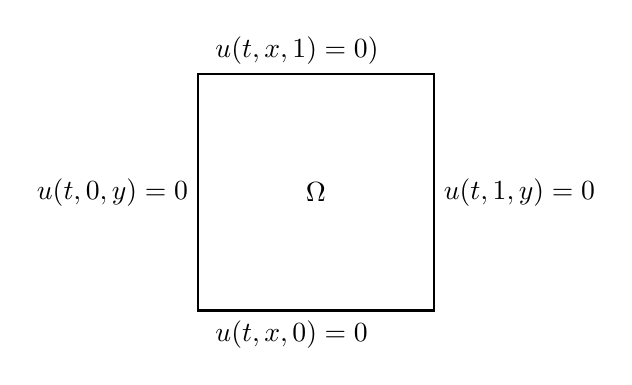
\begin{tikzpicture}
            \draw[thick, black] (0,0) -- (3,0) -- (3,3) -- (0,3) -- cycle;
            \draw (1.5,1.5) node{$\Omega$};
            \draw (0.1,0) node[anchor=north west]{$u(t,x,0) = 0$};
            \draw (0.1,3) node[anchor=south west]{$u(t,x,1) = 0)$};
            \draw (3,1.5) node[anchor=west]{$u(t,1,y)=0$};
            \draw (0,1.5) node[anchor=east]{$u(t,0,y)=0$};
        \end{tikzpicture}
        \caption{Dirichlet boundary conditions for a 2D Poisson equation.}
        \label{fig:2DHeat_BC}
    \end{figure}
    For simplicity we suggest that you take $\Delta x = \Delta y$.  You should also be
    very careful of the stability conditions for the heat equation.  
\end{problem}

\begin{problem}
    Repeat the previous exercise with different boundary conditions (both Dirichlet and
    Neumann) and with different domains (rectangular instead of square).  For a
    rectangular domain it will likely be necessary to have different values for $\Delta
    x$ and for $\Delta y$. Be prepared to present your solutions to your classmates.
\end{problem}

\newpage\section{1D and 2D Wave Equation}
\begin{problem}
   The problems that we've dealt with thus far all model natural diffusion processes: heat
   transport, molecular diffusion, etc.  Another interesting physical phenomenon is that
   of wave propagation.  In 1 spatial dimension the {\it wave equation} is 
   \begin{flalign}
       u_{tt} = \alpha^2 u_{xx}
       \label{eqn:wave1D}
   \end{flalign}
   where $\alpha$ is the stiffness of the wave.  With Dirichlet boundary conditions we can
   think of this as the behaviour of a guitar string after it has been plucked.  

   Let's write MATLAB code to numerically solve this problem:\\
   Consider $u_{tt} = 2 u_{xx}$ in $x \in (0,1)$ with $u(0,x) = x(1-x)$, $u_t(0,x) = 0$,
   and $u(t,0) = u(t,1) = 0$ and $\alpha = 5$.  We can discretize the derivatives as 
   \begin{flalign*}
       u_{tt}(t_{n+1},x_j) &\approx \frac{U_j^{n+1} - 2U_j^n + U_j^{n-1}}{\Delta t^2} \\
       u_{xx}(t_n,x_j) &\approx \frac{U_{j+1}^n - 2U_j^n + U_{j-1}^n}{\Delta x^2}
   \end{flalign*}
\end{problem}

\begin{problem}
    There is a natural stability question waiting to be asked about the discretization of
    the 1D wave equation.  Ask and answer this question.
\end{problem}

\begin{problem}
    In Figure \ref{fig:2DWave_BC} you will see a schematic of the domain
    $\Omega=(0,1)\times (0,1)$ with homogeneous Dirichlet boundary conditions.  Write code
    to solve the 2D Dirichlet problem
    \[ \text{Solve: } u_{tt} = \alpha^2 \nabla \cdot \nabla u  \quad \text{in} \quad x \in \Omega \quad \text{with} \quad
    u(0,x,y) = \sin(2\pi (x-0.5))\sin(2\pi(y-0.5)) \]
    subject to the boundary conditions in the figure.

    \begin{figure}[ht!]
        \centering
        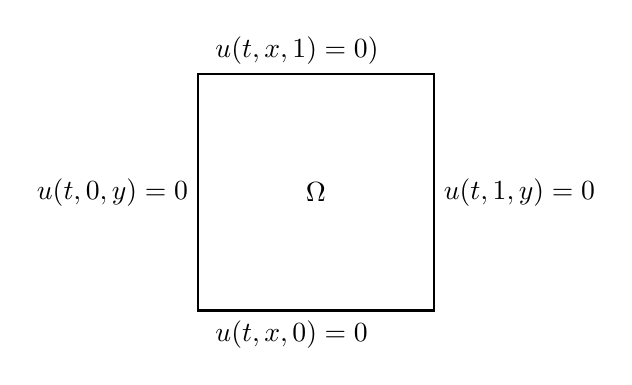
\begin{tikzpicture}
            \draw[thick, black] (0,0) -- (3,0) -- (3,3) -- (0,3) -- cycle;
            \draw (1.5,1.5) node{$\Omega$};
            \draw (0.1,0) node[anchor=north west]{$u(t,x,0) = 0$};
            \draw (0.1,3) node[anchor=south west]{$u(t,x,1) = 0)$};
            \draw (3,1.5) node[anchor=west]{$u(t,1,y)=0$};
            \draw (0,1.5) node[anchor=east]{$u(t,0,y)=0$};
        \end{tikzpicture}
        \caption{Dirichlet boundary conditions for a 2D Poisson equation.}
        \label{fig:2DWave_BC}
    \end{figure}
    For simplicity we suggest that you take $\Delta x = \Delta y$.  You should also be
    very careful of the stability conditions for the heat equation.  
\end{problem}


\newpage\section{Traveling Waves}

\begin{problem}
    A traveling wave can be modeled by the PDE
    \[ u_t + v u_x = 0 \]
    where $v$ is the speed of the wave propogation and $u(t,x)$ is the height of the wave.
    Write a numerical solve for the traveling wave problem on $x \in (0,\infty)$ with initial condition $u(0,x)
    = \text{exp}\left( -\frac{(x-1)^2}{0.1} \right)$, boundary condition $u(t,0) = 0$, and $a=1$.

    Solve this problem with and Euler-type time step and
    \begin{enumerate}
        \item centered differences in space, and
        \item upwind differences in space.
    \end{enumerate}
    where the ``wind'' is from left to right.  Plot both solutions on top of each
    other.  What do you notice about the behavior of the solutions?  Neither of these
    solutions should actually give a traveling wave, but that is what is
    expected out of the solution.  

    {\bf Note about the analytic solution:} If $\eta(x)$ is the initial condition for $u_t + v u_x = 0$ then
    $u(t,x) = \eta(x-vt)$ is the analytic solution to the PDE.  You should check this
    using the chain rule.
\end{problem}


\begin{problem}
    Three ways to fix the issues seen in the previous problem are the ``Leapfrog'' scheme,
    the ``Lax-Friedrichs'' scheme, and the ``Lax-Wendroff'' scheme:
    \begin{flalign}
        \text{Leapfrog: } & \frac{U_j^{n+1} - U_j^{n-1}}{2\Delta t} = -v
        \frac{U_{j+1}^n - U_{j-1}^n}{2\Delta x}
        \label{eqn:frog} \\
        \text{Lax-Friedrichs: } & \frac{U_j^{n+1} - \frac{1}{2} \left( U_{j+1}^n +
        U_{j-1}^n \right)}{\Delta t} = -v \frac{U_{j+1}^n - U_{j-1}^n}{2\Delta x}
        \label{eqn:fried} \\
        \text{Lax-Wendroff: } & U_j^{n+1} = U_j^n - \frac{v \Delta t}{2\Delta x} \left(
        U_{j+1}^n - U_{j-1}^n
        \right) + \left( \frac{v^2 \Delta t^2}{2\Delta x^2} \right) \left( U_{j-1}^n - 2
        U_j^n + U_{j+1}^n.
        \right) \label{eqn:wend}
    \end{flalign}
    Implement all of these schemes and discuss stability and consistency.
\end{problem}


% *******************************


\newpage\section{1D and 2D Steady State PDEs}
\begin{problem}
    Consider a 1-dimensional rod that is infinitely thin and has unit length.  For the
    sake of simplicity assume the following:
    \begin{itemize}
        \item the specific heat of the rod is exactly 1 for the entire length of the rod,
        \item the temperature of the left end is held fixed at $u(0) = 1$,
        \item the temperature of the right end is held fixed at $u(1) = 0$, and
        \item the temperature has reached a steady state.
    \end{itemize}
    (assume that the temperatures are {\it reference temperatures} instead of absolute
    temperatures).

    Since there are no external sources of heat we model the steady-state heat profile
    with Laplace's equation \eqref{eqn:laplace}.  Write this equation in terms of
    1-dimensional spatial derivatives and solve for the temperature profile by hand.
\end{problem}

\begin{problem}
    Devise a way to approximate the temperature profile from the previous problem
    numerically.  Recall that we already know how to build numerical second derivatives.
    Your method will eventually involve solving a system of linear equations.
\end{problem}

\begin{problem}
    Now we will solve the steady state temperature profile problem assuming that there is
    an external source of heat.  This means that we need to solve the 1D Poisson equation
    \eqref{eqn:poisson}.  Take $f(x) = 5\sin(2 \pi x)$, $u(0) = 2$ and $u(1) = 0.5$.
    \[ \text{Solve: } \quad u_{xx} = -5\sin(2\pi x) \quad \text{on} \quad x \in (0,1)
    \quad \text{with} \quad u(0)=2 \quad \text{and} \quad u(1) = 0.5 \]
    First do so by discretizing the domain with very few points so we can write the system
    of equations by hand.  Write your code with the number of points as a parameter so you
    can later change it to several hundred points.
\end{problem}

\begin{problem}
    Generalize the previous problem with a MATLAB function that solves the 1D Poisson
    boundary valued equation:
    \[ \text{Solve: } u_{xx} = - f(x) \quad \text{on} \quad x \in (x_0,x_n) \quad \text{with} \quad
    u(x_0) = \alpha \quad \text{and} \quad u(x_n) = \beta. \]
\begin{lstlisting}
function [x,u] = Poisson1D(f , xmin , xmax , num_interior_pts , BCleft , BCright)
\end{lstlisting}
    Test your code with a known function $f(x)$.

    Note: when we are using fixed values for the boundary conditions these are called
    ``Dirichlet boundary conditions.''
\end{problem}



\begin{problem}
The previous problems only account for Dirichlet boundary conditions (fixed boundary
conditions).  We would now like to modify our Poisson solution to allow for a Neumann
condition: where we know the derivative of $u$ at one of the boundaries.  The
statement of the problem is as follows:
    \[ \text{Solve: } u_{xx} = - f(x) \quad \text{on} \quad x \in (x_0,x_n) \quad \text{with} \quad
    \frac{du}{dx}\Big|_{x_0} = \alpha \quad \text{and} \quad u(x_n) = \beta. \]
    Write a function to solve this problem:
\begin{lstlisting}
function [x,u] = Poisson1D_Neumann(f , xmin , xmax , num_interior_pts , NBC , DBC)
\end{lstlisting}

    Write a MATLAB script to solve the Neumann problem with $f(x) = 2e^{-0.1x}$, $u'(0)=0$,
    and $u(1)=0$.
\end{problem}

\begin{problem}
    Now let's ramp up our discussion of the Poisson equation to two spatial dimensions.
    In Figure \ref{fig:2DPoisson_BC} you will see a schematic of the domain
    $\Omega=(0,1)\times (0,1)$ with Dirichlet boundary conditions.  With the help of your
    instructor, write code to solve the 2D Dirichlet problem
    \[ \text{Solve: } \nabla \cdot \nabla u = - f(x) \quad \text{in} \quad x \in \Omega \quad \text{with} \quad
    f(x,y) = 20\text{exp}\left( -\frac{(x-0.5)^2 + (y-0.5)^2}{0.05} \right) \]
    subject to the boundary conditions in the figure.

    \begin{figure}[ht!]
        \centering
        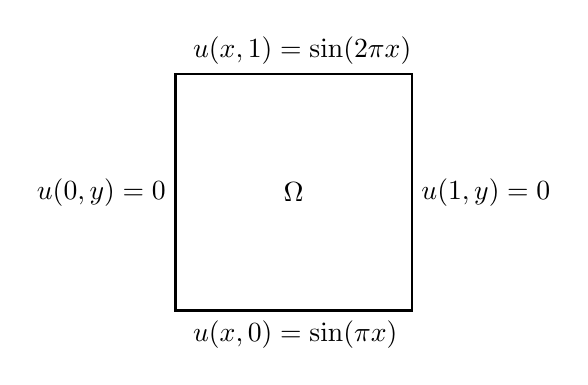
\begin{tikzpicture}
            \draw[thick, black] (0,0) -- (3,0) -- (3,3) -- (0,3) -- cycle;
            \draw (1.5,1.5) node{$\Omega$};
            \draw (0.1,0) node[anchor=north west]{$u(x,0) = \sin(\pi x)$};
            \draw (0.1,3) node[anchor=south west]{$u(x,1) = \sin(2 \pi x)$};
            \draw (3,1.5) node[anchor=west]{$u(1,y)=0$};
            \draw (0,1.5) node[anchor=east]{$u(0,y)=0$};
        \end{tikzpicture}
        \caption{Dirichlet boundary conditions for a 2D Poisson equation.}
        \label{fig:2DPoisson_BC}
    \end{figure}
\end{problem}






\newpage\section{Exercises}

\begin{problem}
    For every one of the scenarios described in Problem \ref{prob:heat_bc}, propose a
    sensible initial condition and solve the problem numerically.  Notice that the
    diffusion coefficient, $D$, is set to 1 for all of these models.  You are welcome to
    change $D$ if you see that it is necessary.
\end{problem}

\begin{problem}
    For every one of the scenarios described in Problem \ref{prob:wave_bc}, propose a
    sensible initial condition and solve the problem numerically.  Notice that the
    tension coefficient, $\alpha^2$, is set to 1 for all of these models.  You are welcome to
    change $\alpha^2$ if you see that it is necessary.
\end{problem}

\begin{problem}
    In this problem we will solve a more realistic 1D heat equation.  We will allow the
    diffusivity to change spatially, so $D = D(x)$ and we want to solve
    \[ u_t = \left( D(x) u'(x) \right)' \]
    on $x \in (0,1)$ with Dirichlet boundary conditions $u(t,0) = u(t,1) = 0$ and initial
    condition $u(0,x) = \sin(2 \pi x)$. In this problem we will take $D(x)$ to be the
    parabola $D(x)= x(1-x)$. We start by doing some calculus to rewrite the
    differential equation:
    \[ u_t = D(x) u''(x) + D'(x) u'(x). \]

    Your jobs are:
    \begin{enumerate}
        \item[(a)] Describe what this choice of $D(x)$ might mean physically in the heat
            equation.
        \item[(b)] Write an explicit scheme to solve this problem by using centered differences
            for the spatial derivatives and an Euler-type discretization for the temporal
            derivative.  Write a clear and thorough explanation for how you are doing the
            discretization as well as a discussion for the errors that are being made with
            each discretization.
        \item[(c)] Write a MATLAB script to find an approximate solution to this problem.
        \item[(d)] Write a clear and thorough discussion about how your will choose $\Delta x$
            and $\Delta t$ to give stable solutions to this equation.
        \item[(e)] Graphically compare your solution to this problem with a heat equation
            where $D$ is taken to be the constant average diffusivity found by calculating
            $D_{ave} = \int_0^1 D(x) dx.$  How does the changing diffusivity change the
            shape of the solution?
    \end{enumerate}

\end{problem}
\hint{
    Since you are solving the heat equation you should be using centered finite
    differences.
}

\begin{problem}[The Diffusing Logo]
    In a square domain create a function $u(0,x,y)$ that looks like your college logo.
    The simplest way to do this might be to take a photo of the logo, crop it to a square,
    and use the \mcode{imread} command to read in the image.  Use this function as the
    initial condition for the heat equation on a square domain with homogeneous Dirichlet
    boundary conditions.  Numerically solve the heat equation and show an animation for
    what happens to the logo as time evolves.
\end{problem}

\begin{problem}[The Wiggling Logo]
    Repeat the previous exercise but this time solve the wave equation with the logo as the
    initial condition.
\end{problem}




\begin{problem}
    Let $u$ be a function modeling a mobile population that in an environment where it has a growth rate of
    $r\%$ per year with a carrying capacity of $K$.  If we were only worried about the
    size of the population we could solve the differential equation 
    \[ \frac{du}{dt} = ru \left( 1-\frac{u}{K} \right), \]
    but there is more to the story.  
    
    Hunters harvest $h$\% of the population per year so we can append the differential
    equation with the harvesting term ``$-h u$'' to arrive at the ordinary differential
    equation 
    \[ \frac{du}{dt} = ru \left( 1-\frac{u}{K} \right) - hu. \]

    Since the population is mobile let's make a few assumptions about the environment that
    they're in and how the individuals move.
    \begin{itemize}
        \item Food is abundant in the entire environment.
        \item Individuals in the population like to spread out so that they don't
            interfere with each other's hunt for food.
        \item It is equally easy for the individuals to travel in any direction in the
            environment.
    \end{itemize}
    Clearly some of these assumptions are unreasonable for real populations and real
    environments, but let's go with it for now.  Given the nature of these assumptions we
    assume that a diffusion term models the spread of the individuals in the population.
    Hence, the PDE model is
    \[ \pd{u}{t} = ru\left( 1-\frac{u}{K} \right) - hu + D \nabla \cdot \nabla u. \]
    \begin{enumerate}
        \item[(a)] Use any of your ODE codes to solve the ordinary differential equation
            with harvesting.  Give a complete description of the parameter space.
        \item[(b)] Write code to solve the spatial+temporal PDE equation on the 2D domain
            $(x,y) \in [0,1] \times [0,1]$.  Choose an appropriate initial condition and
            choose appropriate boundary conditions.
        \item[(c)] The third assumption isn't necessary true for rough terrain. The true
            form of the spatial component of the differential equation is $\nabla \cdot
            \left( D(x,y) \nabla u \right)$ where $D(x,y)$ is a multivariable function
            dictating the ease of diffusion in different spatial locations.  Propose a
            (non-negative) function $D(x,y)$ and repeat part (b) with this new diffusion
            term.
    \end{enumerate}
\end{problem}
\hint{
    Maybe the simplest initial condition for the PDE in part (b) is to use a Gaussian {\it
    bump} that puts the majority of the initial population near the center of the domain.
}


\begin{problem}
    Consider the time-independent partial differential equation $-\varepsilon u_{xx} +
    u_x = 1$ on the domain $x \in (0,1)$ with boundary conditions $u(0) = u(1) = 0$ and
    parameter $\varepsilon$ with $0.001<\varepsilon<1$.
    Write code to solve this boundary valued problem and provide plots of your numerical
    solution for various values of $\varepsilon$. 
\end{problem}


\begin{problem}
    Suppose that we have a concrete slab that is 10 meters in length, with the left
    boundary held at a temperature of $75^\circ$ and the right boundary held at a
    temperature of $90^\circ$.  Assume that the thermal diffusivity of concrete is about
    $k = 10^{-5}$ m$^2$/s.  Assume that the initial temperature of the slab is given by
    the function $T(x) = 75 + 1.5x - 20 \sin( \pi x / 10)$.  In this case, the temperature
    can be analytically solved by the function $T(x,t) = 75 + 1.5x - 20 \sin(\pi x / 10)
    e^{-ct}$ for some value of $c$.  
    \begin{enumerate}
        \item[(a)] Working by hand (no computers!) test this function by substituting it
            into the 1D heat equation and verifying that it is indeed a solution.  In
            doing so you will be able to find the correct value of $c$.
        \item[(b)] Write numerical code to solve this 1D heat equation.  The output of
            your code should be an animation showing how the error between the numerical
            solution and the analytic solution evolve in time.
    \end{enumerate}
\end{problem}

\begin{problem}
    Adobe houses, typically built in desert climates, are known for their great thermal
    efficiency.  The heat equation 
    \[ \frac{\partial T}{\partial t} = \frac{k}{c_p \rho} \nabla \cdot \nabla T, \]
    where $c_p$ is the specific heat of the adobe, $\rho$ is the mass density of the
    adobe, and $k$ is the thermal conductivity of the adobe, can be used to model the heat
    transfer through the adobe from the outside of the house to the inside.  Clearly, the
    thicker the adobe walls the better, but there is a trade off to be considered: 
    \begin{itemize}
        \item it would be prohibitively expensive to build walls so think that the inside
            temperature was (nearly) constant, and 
        \item if the walls are too thin then the cost is low but the temperature inside
            has a large amount of variability.  
    \end{itemize}
    Your Tasks:
    \begin{enumerate}
        \item[(a)] Pick a desert location in the southwestern US (New Mexico, Arizona, Nevada, or
            Southern California) and find some basic temperature data to model the outside
            temperature during typical summer and winter months.
        \item[(b)] Do some research on the cost of building adobe walls and find approximations for the
            parameters in the heat equation.
        \item[(c)] Use a numerical model to find the optimal thickness of an adobe wall.
            Be sure to fully describe your criteria for optimality, the initial and
            boundary conditions used, and any other simplifying assumptions needed for your model.
    \end{enumerate}
\end{problem}
